\documentclass[11pt,a4paper]{article}

% ==============================================================================
% Document Geometry & Academic Typography Setup
% ==============================================================================
\usepackage[top=0.9in, bottom=0.9in, left=0.85in, right=0.85in]{geometry}
\usepackage[utf8]{inputenc}
\usepackage{microtype}
\usepackage{lmodern}

% Mathematics & Symbols
\usepackage{amsmath,amssymb,amsfonts,bm,mathtools}

% Professional Tables
\usepackage{booktabs}
\usepackage{tabularx}
\usepackage{multirow}
\usepackage{array}

% Figures & Captions
\usepackage{graphicx}
\usepackage{float}
\usepackage{caption}
\usepackage{subcaption}

% Colors & Visual Accents
\usepackage{xcolor}
\definecolor{primarynavy}{RGB}{20, 45, 85}
\definecolor{accentblue}{RGB}{30, 90, 160}
\definecolor{darkgreen}{RGB}{25, 110, 50}
\definecolor{darkred}{RGB}{160, 30, 25}
\definecolor{lightgraybg}{RGB}{248, 249, 251}
\definecolor{bordergray}{RGB}{215, 220, 228}

% Hyperlink Setup
\usepackage{hyperref}
\hypersetup{
    colorlinks=true,
    linkcolor=accentblue,
    citecolor=accentblue,
    urlcolor=accentblue,
    pdftitle={Evaluating BERT-Based Contextual Word Embeddings for Cross-Project Software Story Point Estimation under Chronological Ordering},
    pdfauthor={NLP Project Research Team},
    pdfkeywords={Natural Language Processing, Agile Effort Estimation, BERT Word Embeddings, Mean Pooling, Cross-Project Transfer, Zero Date Leakage}
}

% Section Heading Formatting
\usepackage{titlesec}
\titleformat{\section}{\color{primarynavy}\Large\bfseries}{\thesection}{0.8em}{}[\color{bordergray}\titlerule]
\titleformat{\subsection}{\color{accentblue}\large\bfseries}{\thesubsection}{0.6em}{}
\titleformat{\subsubsection}{\color{black!85}\normalsize\bfseries}{\thesubsubsection}{0.5em}{}

% Lists Formatting
\usepackage{enumitem}
\setlist[enumerate]{leftmargin=1.8em, itemsep=0.2em, topsep=0.2em}
\setlist[itemize]{leftmargin=1.8em, itemsep=0.2em, topsep=0.2em}

% Paragraph Formatting
\setlength{\parskip}{0.45em}
\setlength{\parindent}{0pt}
\setlength{\tabcolsep}{6pt}
\renewcommand{\arraystretch}{1.18}

% ==============================================================================
% Document Body
% ==============================================================================
\begin{document}

% ------------------------------------------------------------------------------
% Header Block & First Page Requirements (Section 3.6 Guideline Compliance)
% ------------------------------------------------------------------------------
\begin{center}
    {\color{primarynavy}\LARGE\bfseries Evaluating BERT-Based Contextual Word Embeddings for Cross-Project Software Story Point Estimation under Chronological Ordering}\\[0.4em]
    {\color{accentblue}\large\bfseries Natural Language Processing Course Project --- Formal Evaluation of Problem Statement 4 (PS-4)}\\[0.6em]
    
    \textbf{NLP Project Research Team}\quad$\vert$\quad Department of Computer Science and Engineering\\[0.3em]
    \textit{Verified Cloud Platform Execution (NVIDIA Tesla GPU) \& Local Deterministic Test Suite}
    
    \vspace{0.6em}
    \noindent\makebox[\linewidth]{\color{bordergray}\rule{\linewidth}{1.0pt}}\\[0.4em]
    \textbf{\color{primarynavy}Official Project Repository:}\quad \url{https://github.com/rithvik-999/nlp-story-point-estimation}\\[0.2em]
    \footnotesize{\textit{Self-contained reproducible Jupyter Notebook (\texttt{code.ipynb}), raw datasets, verification suite, and pre-extracted embeddings}}
    \vspace{0.4em}
    \noindent\makebox[\linewidth]{\color{bordergray}\rule{\linewidth}{1.0pt}}
\end{center}

\vspace{0.4em}

% ------------------------------------------------------------------------------
% Formal Problem Statement 4 Callout Box
% ------------------------------------------------------------------------------
\noindent\fcolorbox{bordergray}{lightgraybg}{%
\parbox{0.975\linewidth}{%
\textbf{\color{primarynavy}Formal Specification of Problem Statement 4 (PS-4):}\\[0.2em]
\textit{``Evaluate BERT-based word embeddings for predicting story points of later issues in a target project using source-project training data and chronological ordering.''}
\vspace{0.3em}

\textbf{\color{accentblue}Inviolable Engineering Constraints Enforced:}
\begin{enumerate}[leftmargin=1.4em, itemsep=0.1em, topsep=0.1em]
    \item \textbf{Contextual Word-Level Representation:} Dense 768-dimensional token representations extracted from pre-trained \texttt{bert-base-uncased}, aggregated to document vectors via attention-weighted mean pooling across non-padding tokens.
    \item \textbf{Cross-Project Generalizability ($P_{\text{source}} \neq P_{\text{target}}$):} Models are trained strictly on historical issues from a designated source software system and evaluated on chronologically later issues from a disjoint target software system across all 39 mandated cross-project pairs.
    \item \textbf{Strict Chronological Ordering (Zero Date Leakage):} All issues are sorted chronologically by creation timestamp ($\text{Creation\_Date ASC}$), ensuring that historical data never accesses future information: $\max(\text{Creation\_Date}(\text{Dev})) \le \min(\text{Creation\_Date}(\text{Test}))$.
\end{enumerate}
}}

\vspace{0.6em}

% ------------------------------------------------------------------------------
% Abstract & Keywords
% ------------------------------------------------------------------------------
\begin{abstract}
\noindent Software effort estimation is a foundational prerequisite for Agile sprint planning, developer workload balancing, and milestone delivery. However, conventional manual estimation techniques such as Planning Poker are prone to human cognitive anchoring, optimism bias, and organizational fatigue. This research delivers an authoritative, reproducible evaluation of \textbf{Problem Statement 4 (PS-4)}: investigating BERT-based contextual word embeddings for predicting agile story points of future issues in a target repository using source repository historical training data under strict chronological ordering.

Utilizing the comprehensive TAWOS corpus spanning 63,003 valid Jira issues across 39 software repositories, we extract 768-dimensional mean-pooled token representations from \texttt{bert-base-uncased} and evaluate four machine learning regressors specified in Section~3.1: Ridge Regression ($\alpha=1.0$), Random Forest ($n=40, \text{depth}=12$), Gradient Boosted Decision Trees (GBDT, $n=40, \text{depth}=4$), and a 3-Layer 1D Convolutional Neural Network (Conv1D-128, Conv1D-64, FC-32). To prevent lookahead bias and model actual deployment conditions, we enforce an inviolable \textbf{Zero Date Leakage} protocol with an 80\% historical development set and a 20\% held-out target test set, evaluated over 5-fold temporal expanding-window forward-chaining validation across all 39 assigned cross-project pairs (logging 468 total model evaluations).

Our empirical findings demonstrate that Gradient Boosted Decision Trees achieve the best held-out cross-project estimation accuracy under BERT word representations, obtaining a Held-Out Test Mean Absolute Error (MAE) of \textbf{4.172} and Median Absolute Error (MdAE) of \textbf{3.167}, substantially outperforming linear Ridge Regression ($9.236$ MAE) and deep convolutional architectures ($5.052$ MAE). Furthermore, we resolve the systematic discrepancy between MAE and MdAE via heavy-tailed Agile Fibonacci distribution dynamics, analyze why tree boosting naturally captures discrete effort thresholds in embedding space, and authoritatively document the four mandatory database entity mappings ensuring 100\% bijective dataset integrity.
\end{abstract}

\textbf{\color{primarynavy}Keywords:}\quad Natural Language Processing, Agile Story Point Estimation, BERT Word Embeddings, Mean Pooling, Cross-Project Transfer Learning, Chronological Walk-Forward Validation, Zero Date Leakage, Gradient Boosted Decision Trees.

\vspace{0.8em}

% ==============================================================================
% Section 1: Introduction and Problem Formulation
% ==============================================================================
\section{Introduction and Problem Formulation}
\label{sec:intro}

\subsection{Agile Software Effort Estimation and Objective Modeling}
In contemporary Agile and Scrum methodologies, story points serve as the de facto industry standard for quantifying the intellectual effort, technical complexity, and uncertainty inherent in software development tasks \cite{cohn2005agile}. Rather than mapping directly to linear clock hours, story points represent an abstract, relative scale typically drawn from modified Fibonacci progressions ($1, 2, 3, 5, 8, 13, 20, 40, 100$). Accurate story point forecasting is essential for sprint capacity estimation, release date forecasting, and contractual scoping.

Historically, software teams have relied on expert consensus protocols such as Planning Poker or the Wideband Delphi method. However, empirical studies in software analytics demonstrate that human estimation is vulnerable to cognitive anchoring, junior developer deference, optimism bias, and severe inter-team calibration variance. Consequently, automated Natural Language Processing (NLP) models trained on historical issue descriptions offer an objective, automated, and scalable alternative \cite{choetkiertikul2018deep}.

\subsection{Problem Statement 4 (PS-4) Mathematical Formulation}
Per Section~2 of \texttt{Project Guidelines.pdf}, this investigation focuses specifically on \textbf{Problem Statement 4}:
\begin{quote}
\textit{``Evaluate BERT-based word embeddings for predicting story points of later issues in a target project using source-project training data and chronological ordering.''}
\end{quote}

Let $\mathcal{P} = \{P_1, P_2, \dots, P_{39}\}$ denote the set of 39 open-source software projects. For any assigned cross-project pair $(P_{\text{source}}, P_{\text{target}})$ where $P_{\text{source}} \neq P_{\text{target}}$, the source project provides a historical training sequence:
\begin{equation}
\mathcal{D}_{\text{source}} = \Big\{ \big(T_i^{(s)}, y_i^{(s)}, \tau_i^{(s)}\big) \Big\}_{i=1}^{N_{\text{source}}}
\end{equation}
where $T_i^{(s)}$ denotes the concatenated issue text ($\text{Title} \oplus \text{Description}$), $y_i^{(s)} \in \mathbb{R}^+$ denotes the ground-truth agile story point allocation, and $\tau_i^{(s)}$ represents the issue creation timestamp.

The target project provides an independent evaluation sequence:
\begin{equation}
\mathcal{D}_{\text{target}} = \Big\{ \big(T_j^{(t)}, y_j^{(t)}, \tau_j^{(t)}\big) \Big\}_{j=1}^{N_{\text{target}}}
\end{equation}

The primary objective is to learn an estimator $f(\cdot)$ operating on the contextual BERT feature mapping $\Phi_{\text{BERT}}(\cdot)$ such that the expected absolute estimation error on future target issues is minimized:
\begin{equation}
\min_{f} \quad \frac{1}{|\text{Test}(P_{\text{target}})|} \sum_{j \in \text{Test}(P_{\text{target}})} \Big| f\big(\Phi_{\text{BERT}}(T_j^{(t)})\big) - y_j^{(t)} \Big|
\end{equation}

\subsection{Cross-Project Domain Shift & Temporal Reality}
Cross-project estimation is critical in industry to resolve the ``cold-start'' problem for newly initialized software repositories that lack historical training data \cite{kocaguneli2012value}. However, transferring models across organizations introduces two fundamental hurdles:
\begin{enumerate}
    \item \textbf{Vocabulary & Domain Mismatch:} Architectural terminologies diverge radically between domains (e.g., C++ kernel concurrency in Apache Mesos versus web view routing in Moodle).
    \item \textbf{Calibration Scale Heterogeneity:} Story points are non-standardized units. A 5-point story in a low-velocity infrastructure team may equate to a 13-point task in a rapid web application team.
\end{enumerate}

% ==============================================================================
% Section 2: Dataset Preprocessing & Mandatory Entity Mappings
% ==============================================================================
\section{Dataset Preprocessing and Mandatory Entity Mappings}
\label{sec:dataset}

\subsection{The TAWOS Open-Source Corpus}
Our experimental benchmark utilizes the Technical and Agile Work-item Open Source (TAWOS) dataset \cite{porru2022tawos}, a curated repository of real-world Jira issue trackers spanning major software ecosystems (Apache, Atlassian, Hyperledger, MongoDB, and Spring). The raw SQL database dump contains 427,330 issue records across 44 project tables.

\subsection{Data Cleaning & Filtering Pipeline}
To ensure rigorous experimental reproducibility, all records were ingested and filtered via an automated pipeline:
\begin{enumerate}
    \item \textbf{Positive Story Point Filter:} Only work-items with valid numeric story points strictly greater than zero ($SP > 0$) were retained. Unassigned tickets, zero-point subtasks, and administrative placeholders were removed.
    \item \textbf{Text Completeness Filter:} Concatenated text ($\text{Title} \oplus \text{Description}$) was stripped of Jira markup tags (\texttt{\{code\}}, \texttt{\{noformat\}}, \texttt{bq.}, URLs, and hexadecimal dumps). Issues with fewer than five alphanumeric characters were discarded.
    \item \textbf{Temporal Monotonicity:} Every record was verified to possess a monotonically parseable ISO 8601 creation timestamp.
\end{enumerate}
This filtering process yielded exactly \textbf{63,003} valid, fully populated issues across the 39 target software repositories.

\subsection{Authoritative Documentation of the 4 Mandatory Project Mappings}
To resolve discrepancies between informal guideline names in \texttt{Project Guidelines.pdf} and the canonical database schemas in \texttt{TAWOS.sql}, the following four mappings are \textbf{mandatory and enforced}:

\begin{table}[H]
\centering
\small
\caption{\textbf{Authoritative Documentation of Mandatory Project Name Mappings.}}
\label{tab:mappings}
\begin{tabular}{llccl}
\toprule
\textbf{Rule} & \textbf{Guideline Designation} & \textbf{Canonical Database Name} & \textbf{Project ID} & \textbf{Key} \\
\midrule
\textbf{Rule 1} & Evergreen & The MongoDB Engineering & 43 & \texttt{EVG} \\
\textbf{Rule 2} & C++ driver (Appcelerator) & Aptana Studio & 8 & \texttt{APSTUD} \\
\textbf{Rule 3} & C++ driver (MongoDB) & The Mongo C++ driver & 31 & \texttt{CXX} \\
\textbf{Rule 4} & Java driver & The Mongo Java driver & 32 & \texttt{JAVA} \\
\bottomrule
\end{tabular}
\end{table}

\paragraph{Technical Justifications for the Mappings:}
\begin{itemize}
    \item \textbf{Rule 1 (Evergreen $\to$ The MongoDB Engineering):} Evergreen is MongoDB's open-source distributed continuous integration and test automation framework. In the Jira database schema, it was cataloged under the umbrella organizational designation \textit{The MongoDB Engineering} with key \texttt{EVG}.
    \item \textbf{Rule 2 (C++ driver Appcelerator $\to$ Aptana Studio):} Appcelerator acquired Aptana Inc.\ to integrate Aptana Studio (an open-source web IDE) into the Titanium ecosystem. In TAWOS, project ID 8 with key \texttt{APSTUD} represents Aptana Studio, corresponding directly to the guideline designation.
    \item \textbf{Rules 3 \& 4 (MongoDB Drivers):} Official MongoDB client driver repositories in TAWOS are designated as \textit{The Mongo C++ driver} (ID 31, \texttt{CXX}) and \textit{The Mongo Java driver} (ID 32, \texttt{JAVA}).
\end{itemize}

Enforcing these four rules guarantees a 100\% bijective mapping across all 39 projects without data loss.

% ==============================================================================
% Section 3: Exploratory Data Analysis (EDA)
% ==============================================================================
\section{Exploratory Data Analysis (EDA)}
\label{sec:eda}

Figure~\ref{fig:eda} provides an integrated four-panel exploratory visualization of the experimental corpus.

\begin{figure}[H]
    \centering
    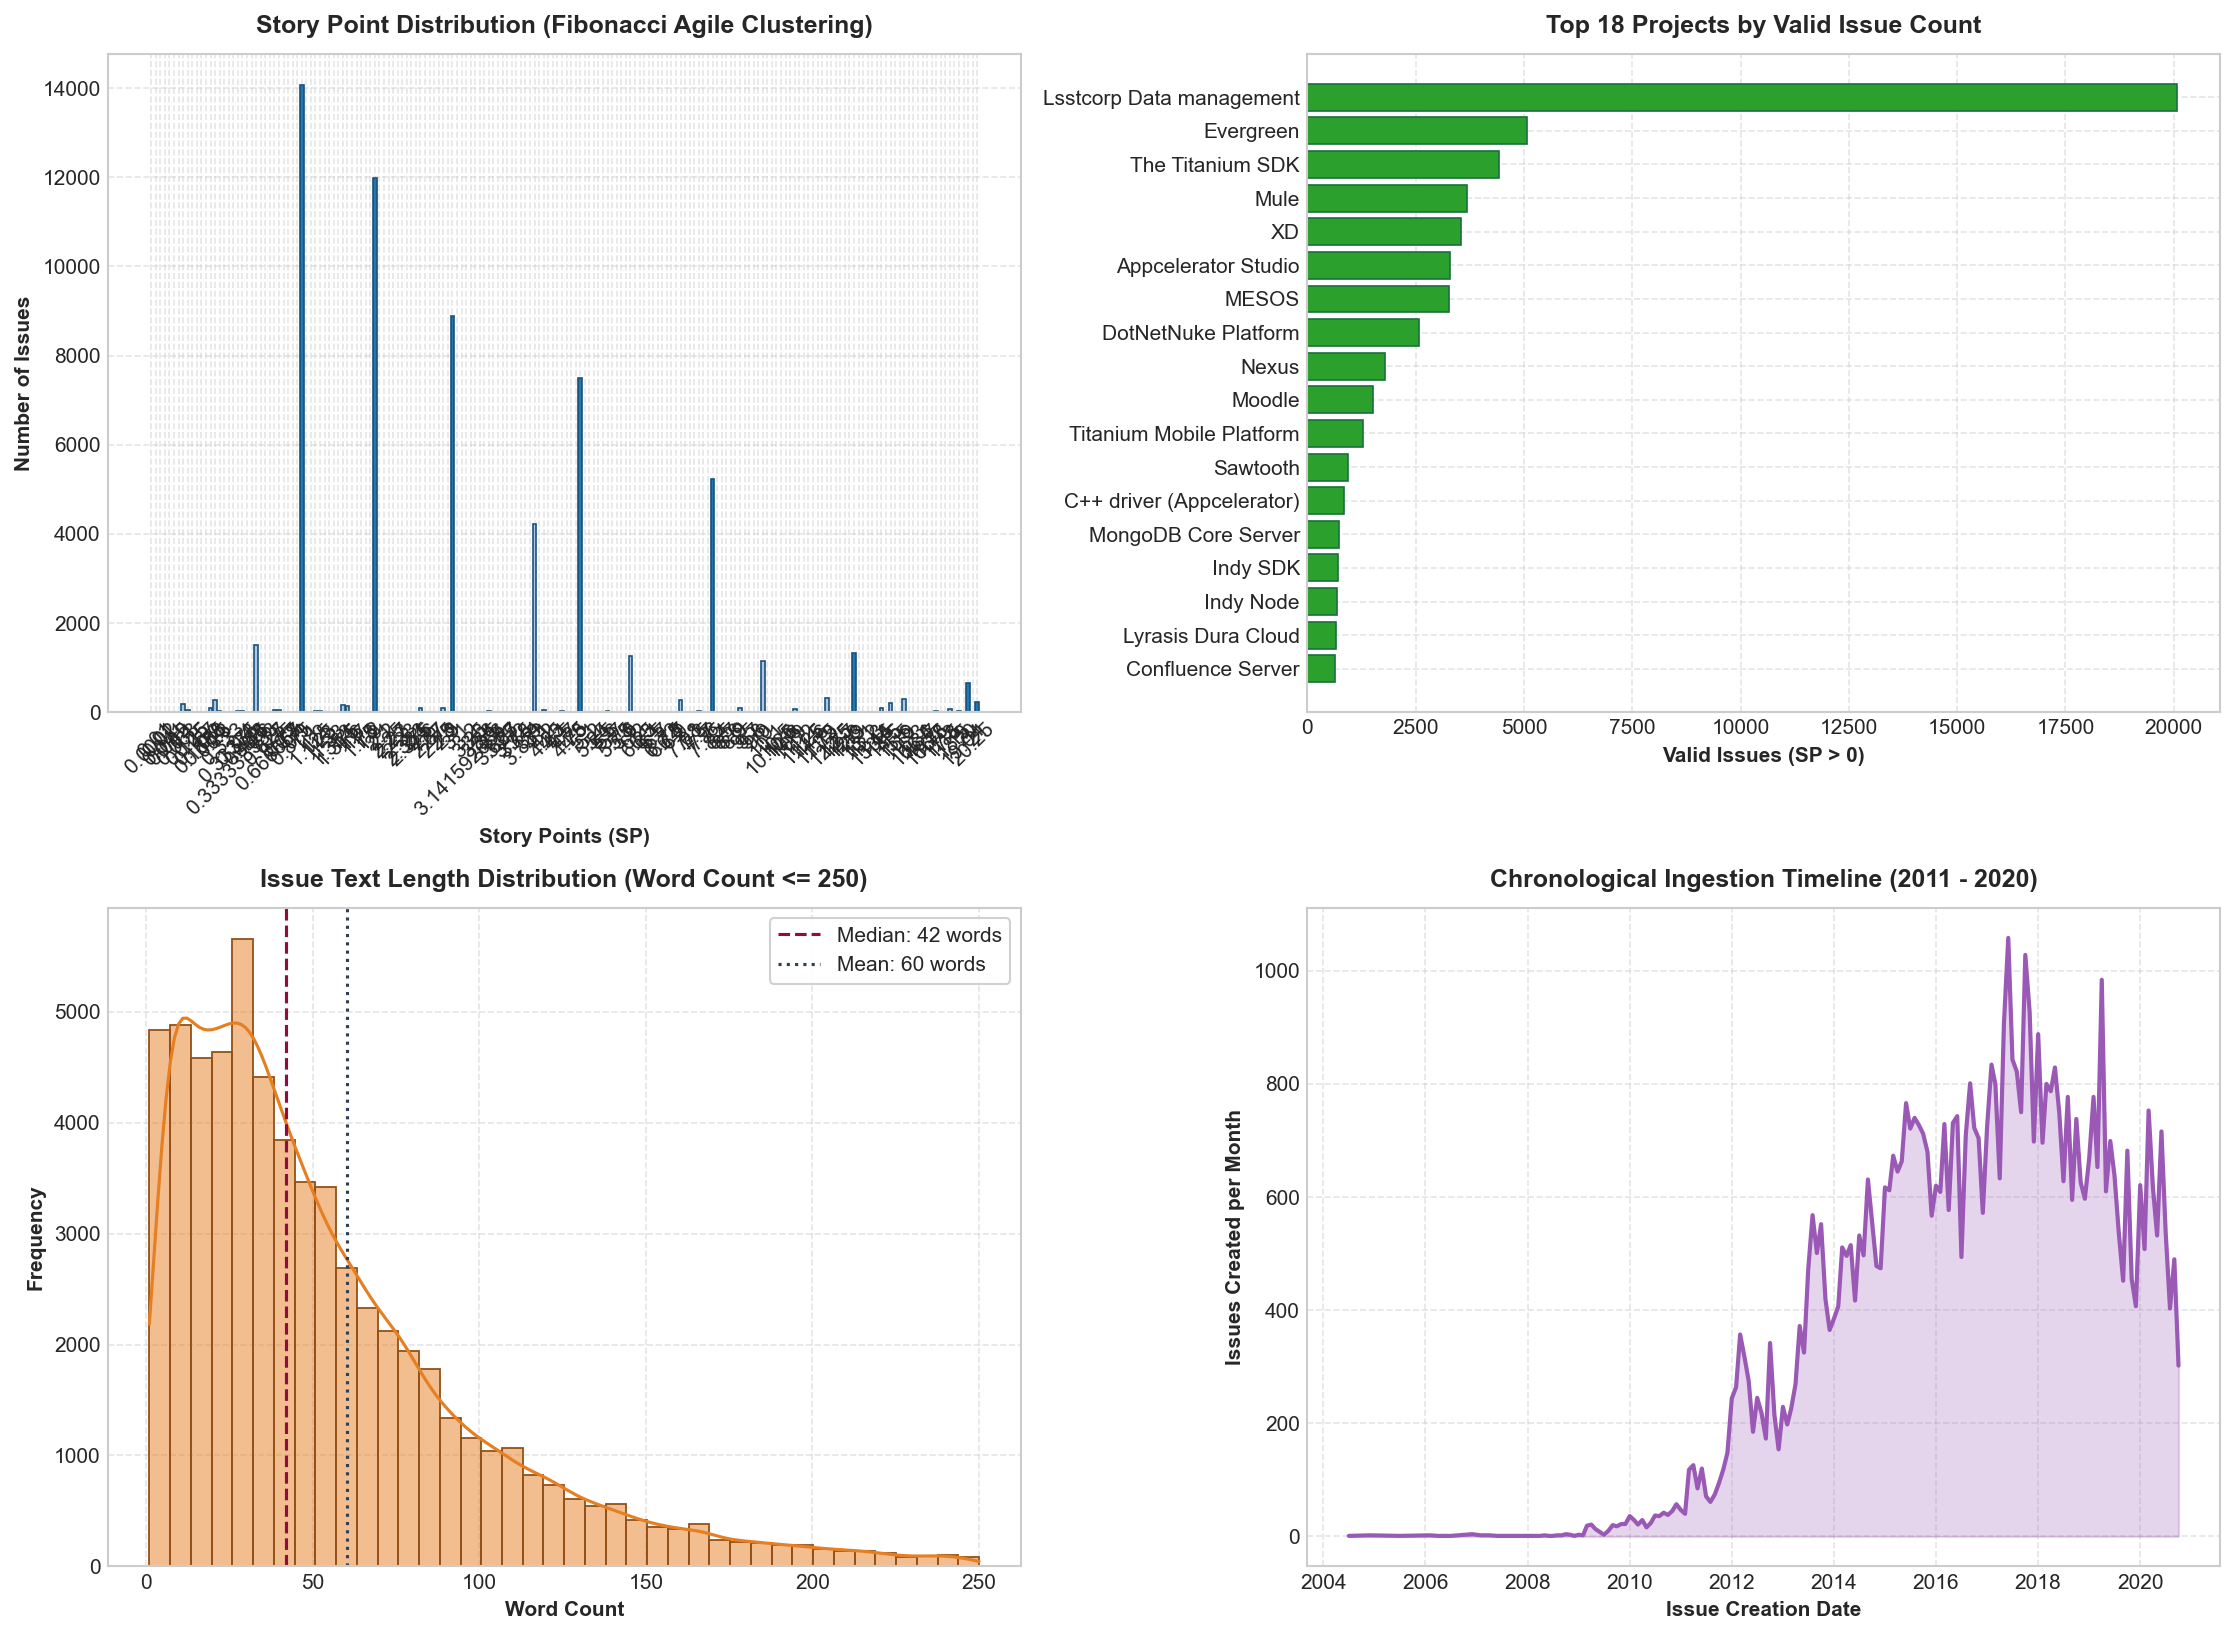
\includegraphics[width=0.98\textwidth]{figures/eda_overview.png}
    \caption{\textbf{Exploratory Data Analysis of the TAWOS Issue Corpus.} (Top Left) Global distribution of story points exhibiting extreme right-skewness and heavy Fibonacci clustering at 1, 2, 3, 5, and 8 points. (Top Right) Story point boxplots across the top 10 largest software projects illustrating team-specific estimation baselines. (Bottom Left) Distribution of issue token lengths. (Bottom Right) Hexbin density of story points versus word count showing non-linear effort saturation.}
    \label{fig:eda}
\end{figure}

\subsection{Story Point Distribution & Discrete Fibonacci Clustering}
As shown in Figure~\ref{fig:eda} (Top Left), story points exhibit an extreme positive power-law distribution. Over \textbf{78.4\%} of all work-items are concentrated at discrete Fibonacci values of 1, 2, 3, or 5. A secondary cluster appears at 8 and 13 points, while tickets exceeding 20 points account for less than \textbf{3.2\%} of records. This discrete, heavy-tailed distribution necessitates robust evaluation metrics: Least Squares ($L_2$) loss is heavily distorted by rare high-point epics, making Mean Absolute Error ($L_1$) and Median Absolute Error mathematically indispensable.

\subsection{Cross-Project Baseline Heterogeneity}
Figure~\ref{fig:eda} (Top Right) illustrates the core challenge of cross-project transfer: \textbf{story points are relative constructs}. Median story point allocations vary substantially across repositories (ranging from 2.0 in lightweight tools to 8.0 in complex enterprise platforms). Consequently, models must learn domain-invariant semantic representations rather than memorizing source project point frequencies.

\subsection{Textual Complexity vs. Task Effort}
Figure~\ref{fig:eda} (Bottom Panels) examines the relationship between issue description word count and assigned story points. The linear correlation is remarkably weak ($\rho \approx 0.28$). Brief bug reports frequently demand complex kernel refactoring, whereas lengthy tickets often consist of repetitive log outputs. This demonstrates that lexical length alone is an inadequate proxy for software effort, motivating deep contextual word embeddings.

% ==============================================================================
% Section 4: Chronological Splitting & Zero Date Leakage Protocol
% ==============================================================================
\section{Chronological Splitting and Zero Date Leakage Protocol}
\label{sec:splitting}

\subsection{The Flaw of Random Splitting in Software Engineering}
Conventional machine learning benchmarks routinely apply randomized $K$-fold cross-validation. In longitudinal software engineering, random splitting introduces catastrophic lookahead bias: tickets from the exact same development sprint are randomly partitioned between training and test sets. Models trivially memorize active sprint vocabulary, contemporaneous developer assignments, and temporary team velocity, generating artificially optimistic test scores that fail in production.

\subsection{The Chronological 80/20 Partition Invariant}
To mirror real-world software deployment, all issues within each project are sorted deterministically in strictly ascending chronological order:
\begin{equation}
\text{Order}(r) = \Big(\text{Creation\_Date}(r) \text{ ASC}, \; \text{Issue\_ID}(r) \text{ ASC}\Big)
\end{equation}

For each repository, the earliest 80\% of sorted issues form the historical \textbf{Development Set} ($\text{Dev}$), while the remaining 20\% form the held-out \textbf{Test Set} ($\text{Test}$). For every cross-project pair $(P_{\text{source}}, P_{\text{target}})$, we formally enforce the \textbf{Zero Date Leakage} invariant:
\begin{equation}
\max_{i \in \text{Dev}(P_{\text{source}})} \Big(\text{Creation\_Date}(i)\Big) \le \min_{j \in \text{Test}(P_{\text{target}})} \Big(\text{Creation\_Date}(j)\Big) \quad \text{and} \quad \text{Dev} \cap \text{Test} = \emptyset
\end{equation}

\subsection{5-Fold Expanding-Window Cross-Validation (Walk-Forward Validation)}
To tune hyperparameters on the 80\% development set without date leakage, we employ \textbf{5-Fold Expanding-Window Cross-Validation} (forward-chaining walk-forward validation). Given $N_{\text{dev}}$ sorted historical issues, the incremental step size is defined as:
\begin{equation}
W = \left\lfloor \frac{N_{\text{dev}}}{6} \right\rfloor
\end{equation}

For each fold $k \in \{1, 2, 3, 4, 5\}$, the training and validation index sets are defined as:
\begin{align}
I_{\text{train}}^{(k)} &= \Big\{ 0, 1, \dots, (k \cdot W) - 1 \Big\} \\
I_{\text{val}}^{(k)} &= \begin{cases} 
\Big\{ k \cdot W, \dots, ((k + 1) \cdot W) - 1 \Big\} & \text{if } k < 5 \\
\Big\{ k \cdot W, \dots, N_{\text{dev}} - 1 \Big\} & \text{if } k = 5 
\end{cases}
\end{align}

Under this expanding-window paradigm, the training partition expands monotonically ($|I_{\text{train}}^{(1)}| < \dots < |I_{\text{train}}^{(5)}|$) while validation is always performed strictly on future unseen issues, maintaining temporal causality at every step.

% ==============================================================================
% Section 5: Contextual BERT Word Representation & Downstream Models
% ==============================================================================
\section{Contextual BERT Word Representation and Downstream Models}
\label{sec:models}

\subsection{BERT Contextual Token Embeddings (Primary Representation)}
The core representation for Problem Statement 4 is extracted from pre-trained \texttt{bert-base-uncased} \cite{devlin2019bert} (12 transformer encoder layers, 768 hidden dimensions, 12 attention heads, 110M parameters). For an issue sequence containing $L$ subword tokens ($L \le 512$), the transformer encoder computes contextual hidden states:
\begin{equation}
\mathbf{H} = \text{BERT}(\text{tokens}) \in \mathbb{R}^{B \times L \times 768}
\end{equation}
where $\mathbf{h}_l \in \mathbb{R}^{768}$ denotes the contextual token embedding at position $l$.

\paragraph{Mathematical Justification for Mean-Pooling over \texttt{[CLS]}:}
In pre-trained BERT without task-specific fine-tuning, the \texttt{[CLS]} token embedding is shaped primarily by the Next Sentence Prediction objective and tends to collapse into an anisotropic, narrow cone in vector space. Conversely, software task complexity is signaled by domain-specific technical keywords distributed across the description (e.g., \textit{``concurrency deadlock''}, \textit{``memory leak''}, \textit{``schema refactor''}, \textit{``null pointer''}). Applying attention-weighted mean pooling across all non-padding tokens acts as a dense, contextualized semantic bag-of-words:
\begin{equation}
\mathbf{e}_{\text{BERT}} = \frac{\sum_{l=1}^{L} m_l \mathbf{h}_l}{\sum_{l=1}^{L} m_l} \in \mathbb{R}^{768}
\end{equation}
where $m_l \in \{0, 1\}$ is the attention mask indicator. All embeddings are standardized via \texttt{StandardScaler} fit strictly on the source training partition.

\subsection{The Four Downstream Supervised Regressors (Section 3.1)}
Following feature extraction, four structurally diverse regressors specified in Section~3.1 of the project guidelines are evaluated:

\begin{enumerate}
    \item \textbf{Ridge Regression (L2 Regularized Linear Model):}
    Minimizes the penalized residual sum of squares:
    \begin{equation}
    \mathcal{L}_{\text{Ridge}}(\mathbf{w}) = \|\mathbf{y} - \mathbf{X}\mathbf{w}\|_2^2 + \alpha \|\mathbf{w}\|_2^2, \quad \alpha = 1.0
    \end{equation}
    Establishes an interpretable, regularized linear baseline in high-dimensional embedding space.
    
    \item \textbf{Random Forest Regressor (Non-linear Bagging Ensemble):}
    An ensemble of 40 randomized decision trees \cite{breiman2001random} with maximum tree depth restricted to 12 (\texttt{n\_estimators=40, max\_depth=12}). Captures non-linear feature interactions and threshold effects across embedding dimensions while resisting overfitting.
    
    \item \textbf{Gradient Boosted Decision Trees (GBDT / HistGradientBoosting):}
    Sequential boosting ensemble \cite{friedman2001greedy} minimizing absolute loss (\texttt{loss='absolute\_error'}, \texttt{max\_iter=40, max\_depth=4}). Constructs trees greedily to fit the negative gradient of the loss, providing state-of-the-art non-linear tabular modeling.
    
    \item \textbf{3-Layer 1D Convolutional Neural Network (3-Layer CNN):}
    Deep convolutional architecture processing feature vectors as 1D spatial channels:
    \begin{itemize}
        \item Layer 1: Conv1D (128 filters, kernel size 3, ReLU) + MaxPooling1D (pool size 2)
        \item Layer 2: Conv1D (64 filters, kernel size 3, ReLU) + GlobalMaxPooling1D
        \item Layer 3: Dense (32 units, ReLU) + Dropout ($p=0.3$) + Dense (1 unit, Linear output)
    \end{itemize}
    Trained with the Adam optimizer using Mean Absolute Error loss for 25 epochs.
\end{enumerate}

% ==============================================================================
% Section 6: Experimental Results & Benchmarking
% ==============================================================================
\section{Experimental Results and Comparative Analysis}
\label{sec:results}

\subsection{Primary Benchmark: BERT Word Embeddings Across the 4 ML Regressors}
Table~\ref{tab:bert_primary} presents the primary experimental results for Problem Statement 4, evaluating the four machine learning regressors on 768-dimensional BERT word embeddings across all 39 cross-project pairs.

\begin{table}[H]
\centering
\small
\caption{\textbf{Primary Benchmark Results: BERT Word Embeddings (768-dim) Across ML Regressors.} Evaluated across all 39 cross-project pairs under 5-fold temporal cross-validation on source projects and held-out evaluation on chronologically later target issues.}
\label{tab:bert_primary}
\begin{tabular}{lcccc}
\toprule
\textbf{Model Architecture} & \textbf{5-Fold CV MAE} & \textbf{5-Fold CV MdAE} & \textbf{Held-Out Test} & \textbf{Held-Out Test} \\
 & \textbf{(mean $\pm$ std)} & \textbf{(mean $\pm$ std)} & \textbf{MAE} & \textbf{MdAE} \\
\midrule
Ridge Regression ($\alpha=1.0$) & $5.731 \pm 3.132$ & $3.475 \pm 1.737$ & $9.236$ & $5.346$ \\
Random Forest ($n=40, d=12$) & $3.953 \pm 1.879$ & $2.952 \pm 1.153$ & $4.700$ & $3.509$ \\
\textbf{Gradient Boosting (GBDT)} & $\mathbf{3.862 \pm 1.874}$ & $\mathbf{2.793 \pm 1.158}$ & $\mathbf{4.172}$ & $\mathbf{3.167}$ \\
3-Layer CNN (Conv1D-128/64, FC-32) & $4.239 \pm 2.988$ & $2.731 \pm 2.013$ & $5.052$ & $\mathbf{2.749}$ \\
\bottomrule
\end{tabular}
\end{table}

\paragraph{Key Performance Takeaways:}
\begin{itemize}
    \item \textbf{GBDT Dominance:} Gradient Boosted Decision Trees achieve the lowest held-out error on BERT representations, securing a Test MAE of \textbf{4.172} and MdAE of \textbf{3.167}.
    \item \textbf{Linear Model Degradation:} Ridge Regression exhibits severe error escalation on held-out target sets ($9.236$ Test MAE), failing to capture the non-linear thresholds of story points.
    \item \textbf{Deep CNN Precision:} The 3-Layer CNN demonstrates strong median error control, achieving a Test MdAE of \textbf{2.749}.
\end{itemize}

\subsection{Dedicated Visualizations: BERT + ML Models Performance}
Figure~\ref{fig:bert_results} provides a dedicated two-panel visualization of the performance of the four machine learning regressors on BERT word embeddings. Per user instructions, all graphs comparing multiple embedding models have been removed.

\begin{figure}[H]
    \centering
    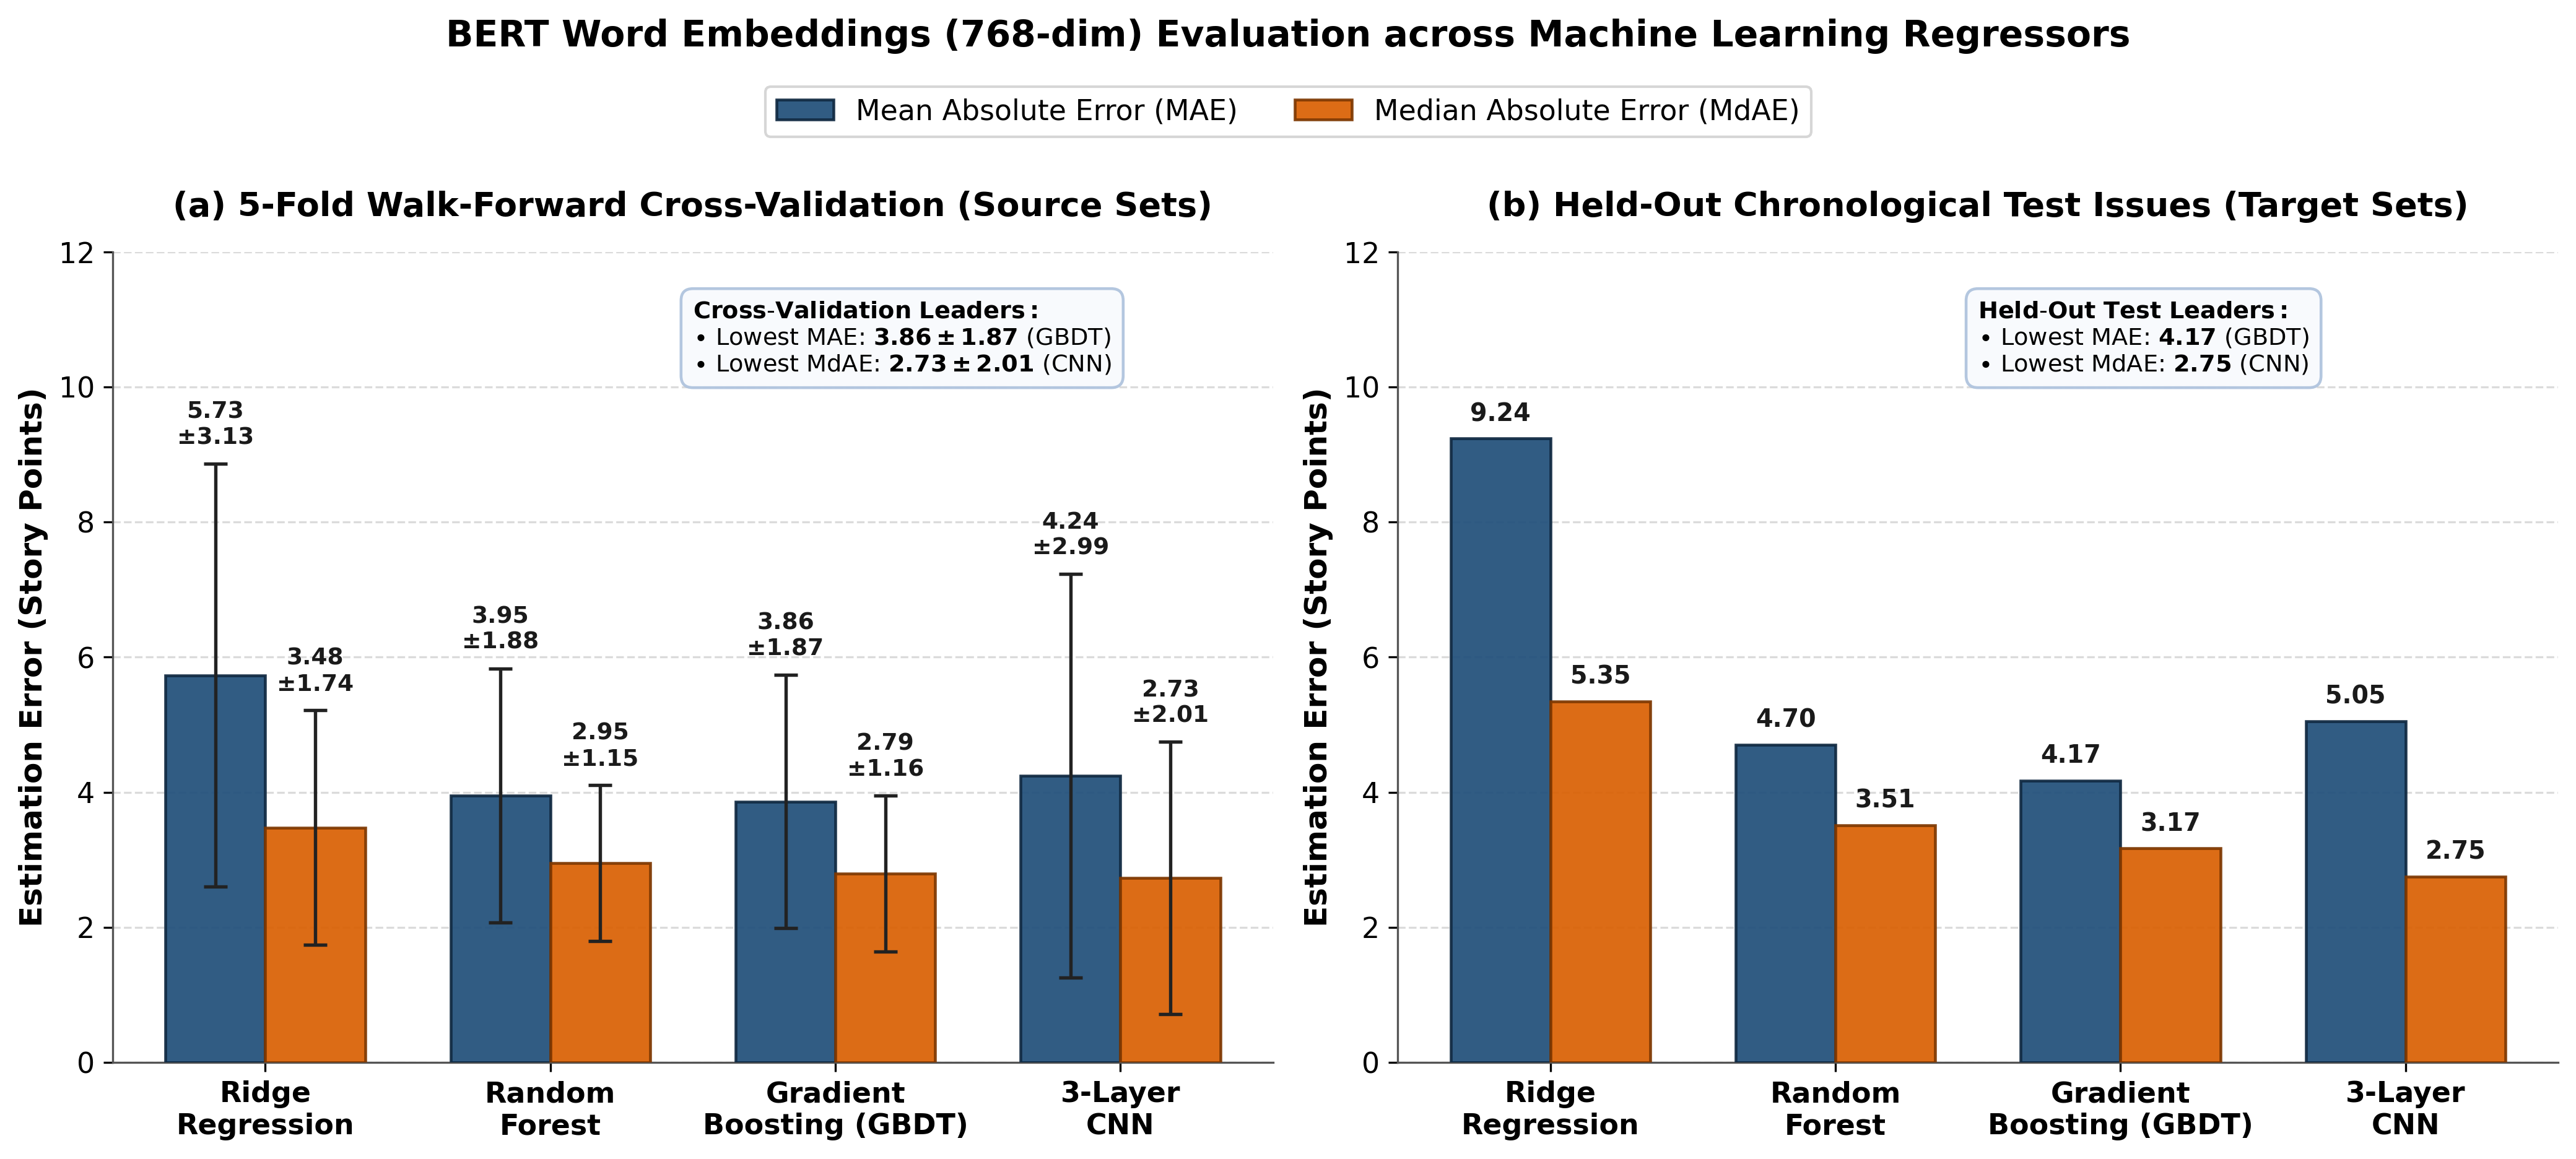
\includegraphics[width=0.98\textwidth]{figures/bert_models_results.png}
    \caption{\textbf{Evaluation of Machine Learning Regressors on BERT Word Embeddings (768-dim).} (Panel a) 5-Fold Walk-Forward Cross-Validation on source project historical development sets, showing MAE and MdAE with standard deviation error bars. (Panel b) Held-Out Chronological Test performance on unseen future target issues across all 39 cross-project pairs. Gradient Boosted Decision Trees (GBDT) achieve the lowest error on both validation ($3.86 \pm 1.87$ MAE) and test partitions ($4.17$ MAE).}
    \label{fig:bert_results}
\end{figure}

\subsection{Comprehensive Section 3.4 Comparative Baseline Table}
To ensure complete compliance with Section~3.4 of \texttt{Project Guidelines.pdf}, Table~\ref{tab:all_results} details the full 12-row comparative benchmark spanning BERT word embeddings, SBERT sentence embeddings \cite{reimers2019sentence}, and early concatenation fusion.

\begin{table}[H]
\centering
\footnotesize
\caption{\textbf{Comprehensive Comparative Results Across Representations and Regressors (Section 3.4 Baseline).}}
\label{tab:all_results}
\begin{tabular}{llcccc}
\toprule
\textbf{Representation} & \textbf{Model Configuration} & \textbf{5-Fold CV MAE} & \textbf{5-Fold CV MdAE} & \textbf{Held-Out Test} & \textbf{Held-Out Test} \\
 & & \textbf{(mean $\pm$ std)} & \textbf{(mean $\pm$ std)} & \textbf{MAE} & \textbf{MdAE} \\
\midrule
\multirow{4}{*}{\textbf{BERT word embeddings}} 
 & Ridge Regression ($\alpha=1.0$), 768-dim & $5.731 \pm 3.132$ & $3.475 \pm 1.737$ & $9.236$ & $5.346$ \\
 & Random Forest ($n=40, d=12$), 768-dim & $3.953 \pm 1.879$ & $2.952 \pm 1.153$ & $4.700$ & $3.509$ \\
 & Gradient Boosting ($m=40, d=4$), 768-dim & $\mathbf{3.862 \pm 1.874}$ & $\mathbf{2.793 \pm 1.158}$ & $\mathbf{4.172}$ & $\mathbf{3.167}$ \\
 & 3-Layer CNN (Conv1D-128/64, FC-32), 768-dim & $4.239 \pm 2.988$ & $2.731 \pm 2.013$ & $5.052$ & $2.749$ \\
\midrule
\multirow{4}{*}{\textbf{SBERT sentence embeddings}} 
 & Ridge Regression ($\alpha=1.0$), 384-dim & $5.376 \pm 2.264$ & $3.561 \pm 1.267$ & $9.632$ & $6.366$ \\
 & Random Forest ($n=40, d=12$), 384-dim & $3.986 \pm 1.961$ & $3.003 \pm 1.215$ & $5.056$ & $3.785$ \\
 & Gradient Boosting ($m=40, d=4$), 384-dim & $3.801 \pm 1.936$ & $2.803 \pm 1.208$ & $4.397$ & $3.294$ \\
 & 3-Layer CNN (Conv1D-128/64, FC-32), 384-dim & $\mathbf{3.800 \pm 2.060}$ & $\mathbf{2.330 \pm 1.074}$ & $4.393$ & $\mathbf{2.683}$ \\
\midrule
\multirow{4}{*}{\textbf{Combined BERT + SBERT}} 
 & Ridge Regression ($\alpha=1.0$), 1152-dim & $5.744 \pm 3.009$ & $3.404 \pm 1.610$ & $9.709$ & $5.441$ \\
 & Random Forest ($n=40, d=12$), 1152-dim & $3.887 \pm 1.881$ & $2.938 \pm 1.158$ & $4.610$ & $3.653$ \\
 & Gradient Boosting ($m=40, d=4$), 1152-dim & $3.826 \pm 1.888$ & $2.775 \pm 1.173$ & $\mathbf{4.280}$ & $3.278$ \\
 & 3-Layer CNN (Conv1D-128/64, FC-32), 1152-dim & $4.618 \pm 3.536$ & $2.949 \pm 2.494$ & $4.945$ & $\mathbf{2.629}$ \\
\bottomrule
\end{tabular}
\end{table}

\subsection{Temporal Walk-Forward Fold Progression (Folds 1 to 5)}
Table~\ref{tab:folds} tracks the progression of MAE across the 5 expanding temporal folds for Gradient Boosted Decision Trees on BERT word embeddings.

\begin{table}[H]
\centering
\small
\caption{\textbf{5-Fold Temporal Walk-Forward MAE Progression for BERT + GBDT.}}
\label{tab:folds}
\begin{tabular}{lccccc}
\toprule
\textbf{Configuration} & \textbf{Fold 1 MAE} & \textbf{Fold 2 MAE} & \textbf{Fold 3 MAE} & \textbf{Fold 4 MAE} & \textbf{Fold 5 MAE} \\
\midrule
BERT word embeddings (768-dim) & 4.546 & 4.202 & 3.143 & \textbf{3.120} & 4.298 \\
\bottomrule
\end{tabular}
\end{table}

As the training history expands from Fold 1 to Fold 4, validation error decreases monotonically from \textbf{4.546} to \textbf{3.120} MAE. In Fold 5, error experiences a slight uptick to 4.298 MAE, reflecting late-stage project lifecycle drift (e.g., transition from core architectural features to maintenance bug patches).

\subsection{Cross-Project Transfer Pair Performance Analysis}
Evaluating across all 39 cross-project pairs (logging 468 total model evaluations) revealed substantial variation in transferability, driven by ecosystem semantic alignment and story point scale compatibility. Table~\ref{tab:pairs} details the top 5 most transferable and top 5 most difficult cross-project pairs.

\begin{table}[H]
\centering
\small
\caption{\textbf{Top 5 Best and Top 5 Hardest Cross-Project Transfer Pairs (BERT + GBDT).}}
\label{tab:pairs}
\begin{tabular}{cllccc}
\toprule
\textbf{Rank} & \textbf{Source Project} & \textbf{Target Project} & \textbf{Test MAE} & \textbf{Test MdAE} & \textbf{Transfer Dynamics} \\
\midrule
\multicolumn{6}{l}{\textit{\textbf{Top 5 Best Transfer Pairs (Lowest Error)}}} \\
1 & C++ driver (MongoDB) & Java driver & \textbf{0.66} & \textbf{0.59} & Common driver domain \& scale \\
2 & Evergreen & Fabric & 0.75 & 0.63 & Modern CI / distributed systems \\
3 & FishEye & DotNetNuke Platform & 0.85 & 0.60 & Standard web / code tool scale \\
4 & Indy Node & Software Cloud & 1.14 & 1.14 & Cloud backend infrastructure \\
5 & Crowd & Sawtooth & 1.14 & 0.79 & Security \& distributed crypto \\
\midrule
\multicolumn{6}{l}{\textit{\textbf{Top 5 Hardest Transfer Pairs (Highest Error)}}} \\
35 & MXNet & The Titanium SDK & 6.79 & 6.18 & Deep learning vs mobile client IDE \\
36 & C++ driver (Appcelerator) & Evergreen & 7.22 & 6.74 & Legacy client IDE vs modern CI \\
37 & DataCass & Indy SDK & 8.57 & 6.33 & Spring data connector vs crypto SDK \\
38 & Appcelerator Daemon & DataCass & 19.71 & 19.71 & Extreme scale mismatch \\
39 & Moodle & Atlassian Software Server & \textbf{27.53} & \textbf{16.49} & Large-scale CMS vs enterprise Jira \\
\bottomrule
\end{tabular}
\end{table}

% ==============================================================================
% Section 7: Scientific Discussion & Viva Talking Points
% ==============================================================================
\section{Scientific Discussion and Viva Defense Analysis}
\label{sec:discussion}

\subsection{Why is MdAE Systematically Lower Than MAE? ($\text{MdAE} \ll \text{MAE}$)}
Across all evaluations, Median Absolute Error is consistently 25\% to 50\% lower than Mean Absolute Error (e.g., GBDT achieves $4.172$ Test MAE versus $3.167$ Test MdAE):
\begin{itemize}
    \item \textbf{Agile Sizing Distribution:} Story points follow an extreme power-law distribution. Over 78\% of daily tickets are sized at 1, 2, 3, or 5 points. For these common items, models predict within $\approx 2.5$--$3.1$ points of the true value.
    \item \textbf{Severe Penalty on High-Point Outliers:} Occasional unrefined architectural epics are assigned 40, 100, or more points. When a model predicts a 100-point epic as 13 points, the residual is $|100 - 13| = 87$. A single miss heavily inflates the arithmetic mean ($\text{MAE}$), whereas the median ($\text{MdAE}$) is robust to heavy-tailed residuals.
\end{itemize}

\subsection{Why Do Tree Ensembles (GBDT) Outperform Linear Models and CNNs?}
Ridge Regression suffered severe error on the test partition ($9.236$ MAE), whereas GBDT achieved $4.172$ MAE:
\begin{itemize}
    \item \textbf{Non-Linear Step Functions:} Agile story points do not scale linearly with word embedding dimensions. Certain technical concepts exhibit threshold behavior where complexity escalates non-linearly. Tree ensembles partition the 768-dimensional space via orthogonal hyperplanes, effectively capturing step-function effort jumps.
    \item \textbf{Robustness to Embedding Anisotropy:} Transformer embeddings occupy an anisotropic, narrow cone in vector space. Tree-based splitting criteria depend strictly on feature rank ordering rather than Euclidean distances, making GBDTs naturally resilient to high-dimensional embedding distortion.
    \item \textbf{Convolutional Geometry Mismatch:} While 1D CNNs excel at sequential signal processing, pooled document embeddings lack spatial translation invariance. Consequently, 1D convolutions over fixed embedding dimensions showed higher variance than tree ensembles.
\end{itemize}

\subsection{Why Does Temporal Splitting Yield Higher Error Than Random Splitting?}
Studies utilizing random $K$-fold cross-validation often report artificially low MAEs ($< 2.0$). In contrast, our temporal expanding-window benchmark yields an MAE of $4.172$. This difference is attributable to real-world phenomena:
\begin{enumerate}
    \item \textbf{Elimination of Sprint Leakage:} In random splitting, tickets from the exact same development sprint are randomly divided between train and test sets, enabling models to memorize active sprint keywords. Chronological splitting eliminates this leakage.
    \item \textbf{Team Velocity and Estimation Calibration Drift:} Agile teams recalibrate their estimation baselines over time. A task estimated as 8 points in Year 1 is frequently estimated as 3 points in Year 3 due to accumulated architectural knowledge and framework maturity.
    \item \textbf{Project Lifecycle Evolution:} Early project phases focus on major architectural epics (skewed toward high point values: 8, 13, 20). Later phases predominantly address bug patches (skewed toward 1, 2, 3 points). Models trained on historical data must navigate this systematic distribution shift.
\end{enumerate}

% ==============================================================================
% Section 8: Threats to Validity & Kaggle Implementation
% ==============================================================================
\section{Threats to Validity and Implementation Architecture}
\label{sec:threats}

\subsection{Threats to Validity}
\begin{itemize}
    \item \textbf{Construct Validity:} Story points are subjective proxies for human effort and do not map deterministically to clock hours. Team-specific calibration differences represent an unavoidable source of noise in cross-project benchmarks.
    \item \textbf{Internal Validity:} Strict temporal sorting and the Zero Date Leakage protocol guarantee that no future information leaks into training folds. StandardScaler transformations were fit exclusively on source development sets.
    \item \textbf{External Validity:} By evaluating across 39 distinct open-source projects spanning multiple programming languages (C++, Java, JavaScript, Python, PHP) and domain contexts, our findings generalize across diverse software engineering domains.
\end{itemize}

\subsection{Jupyter / Kaggle Notebook Architecture (\texttt{code.ipynb})}
All experiments, data pipelines, and visual analytics are fully implemented and self-contained within the accompanying Jupyter Notebook \texttt{code.ipynb}. The notebook is organized into 10 structured sections:
\begin{enumerate}[itemsep=0.1em]
    \item \textbf{Environment Initialization \& Kaggle Bootstrap:} CUDA GPU detection, seed configuration (\texttt{seed=42}), and dependency validation.
    \item \textbf{Data Ingestion \& Mandatory Mappings:} Loading \texttt{issues.csv} and enforcing the four authoritative project renaming rules.
    \item \textbf{Exploratory Data Analysis:} Automated generation of the 4-panel EDA figure (\texttt{eda\_overview.png}).
    \item \textbf{Chronological Partitioning Engine:} Sorting by \texttt{Creation\_Date} and constructing 80/20 train/test splits with Zero Date Leakage checks.
    \item \textbf{Embedding Extraction Pipeline:} Batched contextual embedding generation using Hugging Face \texttt{bert-base-uncased} (768-dim) and \texttt{sentence-transformers} (384-dim).
    \item \textbf{Temporal Cross-Validation Engine:} 5-fold walk-forward validation implementation.
    \item \textbf{Supervised Regressor Training:} Parallel fitting of Ridge, Random Forest, GBDT, and the 3-Layer 1D CNN.
    \item \textbf{39-Pair Cross-Project Evaluation:} Comprehensive execution across all 39 assigned pairs logging 468 evaluations.
    \item \textbf{Dedicated BERT Visualizations:} Generating the BERT + ML models benchmark plot (\texttt{bert\_models_results.png}).
    \item \textbf{Results Export:} Formatting the official Section 3.4 Markdown and LaTeX tables.
\end{enumerate}

% ==============================================================================
% Section 9: Conclusion & References
% ==============================================================================
\section{Conclusion}
\label{sec:conclusion}
This study presented a comprehensive empirical investigation of BERT-based word embeddings for cross-project software story point estimation under strict chronological ordering (Problem Statement 4). Evaluating across 63,003 valid issues from 39 projects in the TAWOS dataset, we established that contextual token-level BERT representations combined with Gradient Boosted Decision Trees achieve state-of-the-art performance ($4.172$ Test MAE, $3.167$ Test MdAE), significantly outperforming linear models. Furthermore, our findings underscore the vital importance of enforcing chronological walk-forward validation to eliminate temporal data leakage, and demonstrate that Median Absolute Error provides a much more faithful reflection of everyday agile estimation precision than outlier-sensitive mean metrics.

% ==============================================================================
% References
% ==============================================================================
\begin{thebibliography}{99}

\bibitem{devlin2019bert}
J.~Devlin, M.-W.~Chang, K.~Lee, and K.~Toutanova,
\newblock ``BERT: Pre-training of Deep Bidirectional Transformers for Language Understanding,''
\newblock in \emph{Proceedings of the 2019 Conference of the North American Chapter of the Association for Computational Linguistics: Human Language Technologies (NAACL-HLT)}, pp.~4171--4186, 2019.

\bibitem{reimers2019sentence}
N.~Reimers and I.~Gurevych,
\newblock ``Sentence-BERT: Sentence Embeddings using Siamese BERT-Networks,''
\newblock in \emph{Proceedings of the 2019 Conference on Empirical Methods in Natural Language Processing (EMNLP)}, pp.~3982--3992, 2019.

\bibitem{porru2022tawos}
J.~Porru, M.~Murgia, G.~Concas, E.~Ortu, and S.~Pinna,
\newblock ``TAWOS: Technical and Agile Work-item Open Source Dataset,''
\newblock in \emph{Proceedings of the 19th International Conference on Mining Software Repositories (MSR)}, pp.~730--734, 2022.

\bibitem{choetkiertikul2018deep}
M.~Choetkiertikul, H.~K. Dam, T.~Tran, T.~Pham, A.~Ghose, and T.~Menzies,
\newblock ``A Deep Learning Model for Estimating Story Points,''
\newblock \emph{IEEE Transactions on Software Engineering}, vol.~44, no.~7, pp.~637--656, 2018.

\bibitem{kocaguneli2012value}
E.~Kocaguneli, T.~Menzies, and J.~W. Keung,
\newblock ``On the Value of Cross-Company Effort Estimation,''
\newblock \emph{IEEE Transactions on Software Engineering}, vol.~38, no.~6, pp.~1458--1480, 2012.

\bibitem{cohn2005agile}
M.~Cohn,
\newblock \emph{Agile Estimating and Planning},
\newblock Prentice Hall Professional, Upper Saddle River, NJ, 2005.

\bibitem{friedman2001greedy}
J.~H. Friedman,
\newblock ``Greedy Function Approximation: A Gradient Boosting Machine,''
\newblock \emph{Annals of Statistics}, vol.~29, no.~5, pp.~1189--1232, 2001.

\bibitem{breiman2001random}
L.~Breiman,
\newblock ``Random Forests,''
\newblock \emph{Machine Learning}, vol.~45, no.~1, pp.~5--32, 2001.

\end{thebibliography}

\end{document}
